\documentclass[conference]{IEEEtran}
\IEEEoverridecommandlockouts
% The preceding line is only needed to identify funding in the first footnote. If that is unneeded, please comment it out.
%----------------------------------------------------------
\usepackage{cite}
\usepackage[pdftex]{graphicx}
\usepackage{siunitx}
% declare the path(s) where your graphic files are
\graphicspath{images/}
\DeclareGraphicsExtensions{.pdf,.jpeg,.png,.jpg}
\usepackage{amsmath,amssymb,amsfonts}
\usepackage{algorithmic}
\usepackage{graphicx}
\usepackage{textcomp}
\usepackage{array}
%\usepackage[caption=false,font=normalsize,labelfont=sf,textfon =sf]{subfig}
\usepackage{dblfloatfix}
\usepackage{url}
\usepackage{lipsum}
\usepackage{listings}
\usepackage{xcolor}
\def\BibTeX{{\rm B\kern-.05em{\sc i\kern-.025em b}\kern-.08em
    T\kern-.1667em\lower.7ex\hbox{E}\kern-.125emX}}
%----------------------------------------------------------
    \lstset{
        escapeinside={/*@}{@*/},
        language=Python,	
        basicstyle=\fontsize{8.5}{12}\selectfont,
        numbers=left,
        numbersep=2pt,    
        xleftmargin=2pt,
        frame=tb,
        columns=fullflexible,
        showstringspaces=false,
        tabsize=4,
        keepspaces=true,
        showtabs=false,
        showspaces=false,
        morekeywords={inline,public,class,private,protected,struct},
        captionpos=b,
        lineskip=-0.4em,
        aboveskip=10pt,
        extendedchars=true,
        breaklines=true,
        prebreak = \raisebox{0ex}[0ex][0ex]{\ensuremath{\hookleftarrow}},
        keywordstyle=\color[rgb]{0,0,1},
        commentstyle=\color[rgb]{0.133,0.545,0.133},
        stringstyle=\color[rgb]{0.627,0.126,0.941},
    }
%----------------------------------------------------------

\begin{document}

\title{Trocando mensagens\\
{\footnotesize \textsuperscript{*} Sistemas Embarcados: Prof. Marco Reis - marco.reis@ba.docente.senai.br}
}

% \author{\IEEEauthorblockN{Marco Reis, 41650-010\IEEEauthorrefmark{1}}
% \IEEEauthorblockA{\IEEEauthorrefmark{1}Robotics & Autonomous Systems Center,
% Senai Cimatec, Salvador, Brazil}% <-this % stops an unwanted space

\author{
    \IEEEauthorblockN\centerline{}{Ludmila Nascimento Dos Anjos}
    \IEEEauthorblockA{\textit{Graduanda em Engenharia Elétrica} \\
        \textit{SENAI CIMATEC}\\
        Salvador, Bahia \\
        ludmila.n.anjos@gmail.com}
    \and
}
\maketitle

\begin{abstract}
    This document is a model and instructions for \LaTeX.
    This and the IEEEtran.cls file define the components of your paper [title, text, heads, etc.]. *CRITICAL: Do Not Use Symbols, Special Characters, Footnotes,
    or Math in Paper Title or Abstract.
\end{abstract}

\begin{IEEEkeywords}
    Arduino, Comunicação Serial, Sistema Embarcado, LCD, Sensor ultrassônico
\end{IEEEkeywords}

\section{Introdução}

\subsection{Contexto}

\subsection{Justificativa}

\subsection{Porquê}

\subsection{Importância}

\subsection{Objetivos}

\section{Referencial teórico}
Nesta seção serão apresentados os dispositivos, e a forma de comunicação, utilizadas para o desenvolvimento do projeto.
\subsection{Arduino}
\subsection{Medição de distância através do Sensor ultrassônico}

\begin{equation}
    distancia = tempo / 27.6233 / 2.0 \label{eq}
\end{equation}

\subsection{Sinalização com LED(Light Emitting Diode)}
\subsection{Display LCD(Liquid crystal display)}
\subsection{Potenciômetro}
\subsection{Comunicação Serial}

\section{Metodologia}

\subsection{Materiais}
Os materiais de hardware utilizados para a elaboração do projeto foram:
\begin{itemize}
    \item 2 arduinos UNO;
    \item 2 protoboards;
    \item 1 potenciômetro;
    \item 1 display de LCD;
    \item 1 sensor ultrassônico HC-SR04;
    \item 32 jumpers;
    \item 1 LED azul;
    \item 1 LED vermelho;
    \item 1 LED amarelo;
    \item 3 resistores de 220 \si{\ohm};
    \item 1 resistor de 1 K \si{\ohm};
\end{itemize}
Os softwares utlizados foram:
\begin{itemize}
    \item Tinkercad;
    \item Arduino IDE;
\end{itemize}

\subsection{Métodos}

Realizou-se as conexões dos dispositivos ao arduino no simulador tinkercad conforme o mostrado na figura 1.
Então, foi efetuada a programação de ambos os arduinos. O arduino 1 foi programado para captar dados do sensor ultrassônico, tratá-los
e conforme a distância em centímetros identificada acender um led azul, vermelho e amarelo para representar a região ao qual se encontra o objeto, sendo que a região mais próxima é a região 3, representada pelo led azul.
Além disso, ele também envia a informação sobre a distância de um objeto como string via comunicação serial para o arduino 2, que por sua vez utiliza de um display lcd, com regulação de brilho via potenciômetro, para mostrar a informação.

Em seguida, após a confecção do modelo virtual foi montado o circuito físico(Figura 2) com os mesmos materiais de hardware e com a mesma programação inserida nos dois arduinos através do software arduino IDE e uma conexão com um notebook.


\begin{figure}[htbp]
    \centerline{
        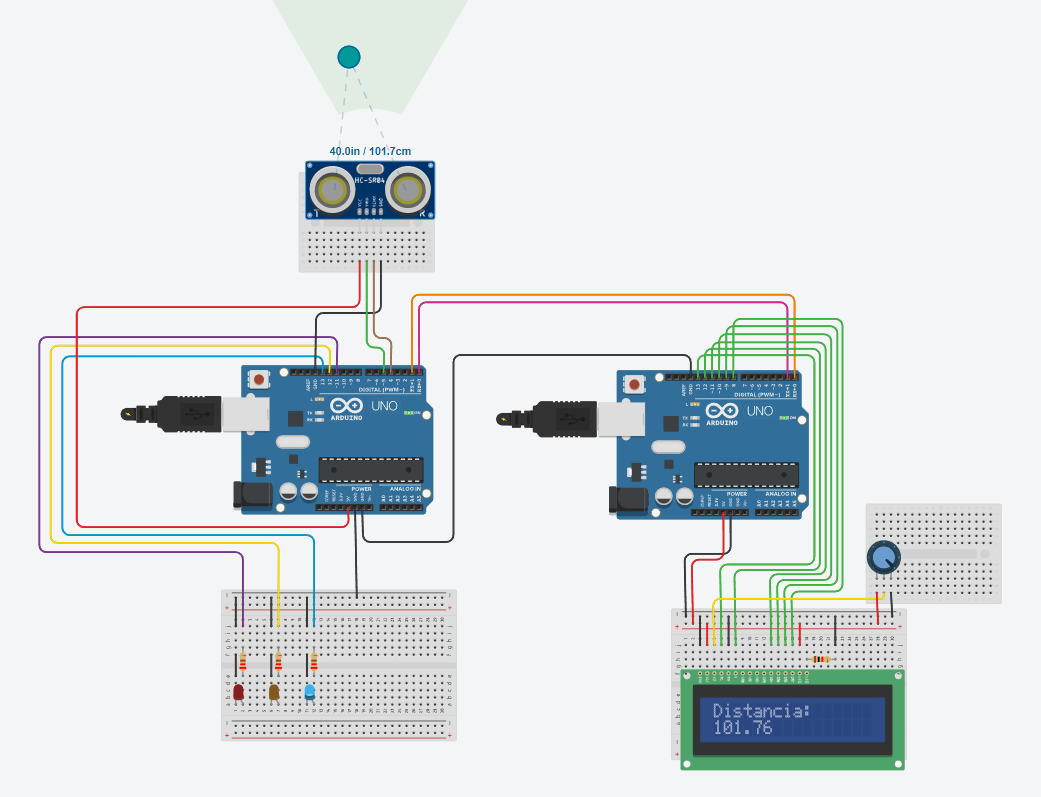
\includegraphics[width=4cm]{images/esquema-arduino.png}
    }
    \caption{Esquematico arduino.}
    \label{fig}
\end{figure}

\begin{figure}[htbp]
    \centerline{
        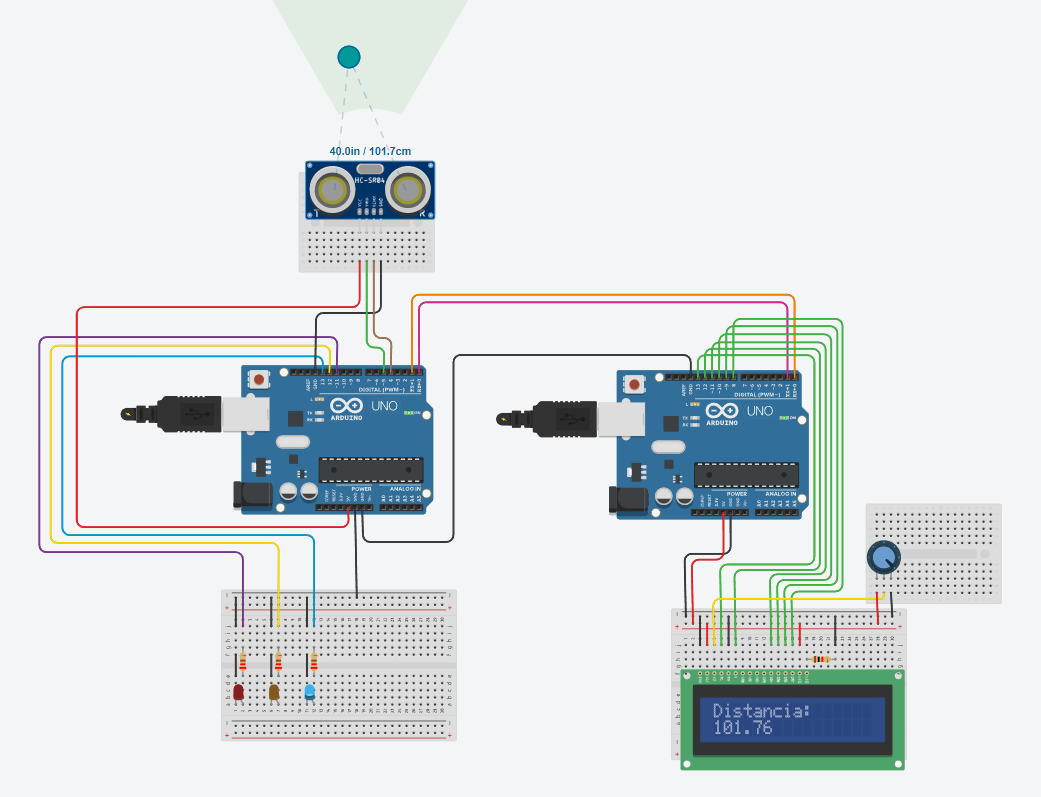
\includegraphics[width=4cm]{images/esquema-arduino.png}
    }
    \caption{Esquematico arduino.}
    \label{fig}
\end{figure}

\section{Resultados e Análises}

\subsection{Montagem do circuito}

Na montagem do esquemático do circuito virtual no simulador Tinkercad não ocorreu nenhuma dificuldade relacionada à conexão entre componentes.
Diferentemente da montagem do circuito físico, pois, devido ao mau contato entre as ligações os dados passados para o display estiveram corrompidos. Para solucionar este problema jumpers precisaram ser substituídos
e o display precisou ser soldado a um suporte para conectá-lo à protoboard.

\subsection{Efeito do delay}
Notou-se que o valor utilizado na função delay afetou drasticamente a comunicação serial entre os dois arduinos, a forma encontrada para contornar isso foi utilizar a função delayMicroseconds. Pois, esta afeta menos ao tempo de comunicação do sistema.

\subsection{Leitura do sensor ultrassônico HC-SR04}

O sistema físico do arduino master ao receber dados referente ao tempo para a captação da reflexão de uma onda de som ultrassônico realizou o cálculo da distância entre o objeto e o sensor.
Foi perceptível a pequena oscilação entre os valores obtidos de distância, isso ocorreu pois o sensor não possuí filtros eletrônicos específicos e estava sujeito a interferência causada por outras ondas sonoras no ambiente.

Devido a essa oscilação, a forma utilizada para diminuir a alteração no valor de distância mostrado no display LCD foi mostrar nele a média de 5 valores lidos.

\section{Conclusão}
Conclui-se que os sensor ultrassônico HC-SR04... Além disso, o mal contato entre os componentes... Dessa forma, o projeto se apresentou como uma excelente forma de compreender o funcionamento de dispositivos eletrônicos e sua comunicação.

\bibliographystyle{IEEEtran}
\bibliography{Bibliography}







\section{Modelos}
Before you begin to format your paper, first write and save the content as a
separate text file. Complete all content and organizational editing before
formatting. Please note sections \ref{AA}--\ref{SCM} below for more information on
proofreading, spelling and grammar.

Keep your text and graphic files separate until after the text has been
formatted and styled. Do not number text heads---{\LaTeX} will do that
for you.

\subsection{Equations}
Number equations consecutively. To make your
equations more compact, you may use the solidus (~/~), the exp function, or
appropriate exponents. Italicize Roman symbols for quantities and variables,
but not Greek symbols. Use a long dash rather than a hyphen for a minus
sign. Punctuate equations with commas or periods when they are part of a
sentence, as in:
\begin{equation}
    a+b=\gamma\label{eq}
\end{equation}

Be sure that the
symbols in your equation have been defined before or immediately following
the equation. Use ``\eqref{eq}'', not ``Eq.~\eqref{eq}'' or ``equation \eqref{eq}'', except at
the beginning of a sentence: ``Equation \eqref{eq} is . . .''

\subsection{\LaTeX-Specific Advice}

Please use ``soft'' (e.g., \verb|\eqref{Eq}|) cross references instead
of ``hard'' references (e.g., \verb|(1)|). That will make it possible
to combine sections, add equations, or change the order of figures or
citations without having to go through the file line by line.

Please don't use the \verb|{eqnarray}| equation environment. Use
\verb|{align}| or \verb|{IEEEeqnarray}| instead. The \verb|{eqnarray}|
environment leaves unsightly spaces around relation symbols.

Please note that the \verb|{subequations}| environment in {\LaTeX}
will increment the main equation counter even when there are no
equation numbers displayed. If you forget that, you might write an
article in which the equation numbers skip from (17) to (20), causing
the copy editors to wonder if you've discovered a new method of
counting.

    {\BibTeX} does not work by magic. It doesn't get the bibliographic
data from thin air but from .bib files. If you use {\BibTeX} to produce a
bibliography you must send the .bib files.

    {\LaTeX} can't read your mind. If you assign the same label to a
subsubsection and a table, you might find that Table I has been cross
referenced as Table IV-B3.

{\LaTeX} does not have precognitive abilities. If you put a
\verb|\label| command before the command that updates the counter it's
supposed to be using, the label will pick up the last counter to be
cross referenced instead. In particular, a \verb|\label| command
should not go before the caption of a figure or a table.

Do not use \verb|\nonumber| inside the \verb|{array}| environment. It
will not stop equation numbers inside \verb|{array}| (there won't be
any anyway) and it might stop a wanted equation number in the
surrounding equation.

\subsection{Some Common Mistakes}\label{SCM}
\begin{itemize}
    \item The word ``data'' is plural, not singular.
    \item The subscript for the permeability of vacuum $\mu_{0}$, and other common scientific constants, is zero with subscript formatting, not a lowercase letter ``o''.
    \item In American English, commas, semicolons, periods, question and exclamation marks are located within quotation marks only when a complete thought or name is cited, such as a title or full quotation. When quotation marks are used, instead of a bold or italic typeface, to highlight a word or phrase, punctuation should appear outside of the quotation marks. A parenthetical phrase or statement at the end of a sentence is punctuated outside of the closing parenthesis (like this). (A parenthetical sentence is punctuated within the parentheses.)
    \item A graph within a graph is an ``inset'', not an ``insert''. The word alternatively is preferred to the word ``alternately'' (unless you really mean something that alternates).
    \item Do not use the word ``essentially'' to mean ``approximately'' or ``effectively''.
    \item In your paper title, if the words ``that uses'' can accurately replace the word ``using'', capitalize the ``u''; if not, keep using lower-cased.
    \item Be aware of the different meanings of the homophones ``affect'' and ``effect'', ``complement'' and ``compliment'', ``discreet'' and ``discrete'', ``principal'' and ``principle''.
    \item Do not confuse ``imply'' and ``infer''.
    \item The prefix ``non'' is not a word; it should be joined to the word it modifies, usually without a hyphen.
    \item There is no period after the ``et'' in the Latin abbreviation ``et al.''.
    \item The abbreviation ``i.e.'' means ``that is'', and the abbreviation ``e.g.'' means ``for example''.
\end{itemize}
An excellent style manual for science writers is \cite{young1989technical}.

\subsection{Figures and Tables}
\paragraph{Positioning Figures and Tables} Place figures and tables at the top and
bottom of columns. Avoid placing them in the middle of columns. Large
figures and tables may span across both columns. Figure captions should be
below the figures; table heads should appear above the tables. Insert
figures and tables after they are cited in the text. Use the abbreviation
``Fig.~\ref{fig}'', even at the beginning of a sentence.

\begin{table}[htbp]
    \caption{Table Type Styles}
    \begin{center}
        \begin{tabular}{|c|c|c|c|}
            \hline
            \textbf{Table} & \multicolumn{3}{|c|}{\textbf{Table Column Head}}                                                         \\
            \cline{2-4}
            \textbf{Head}  & \textbf{\textit{Table column subhead}}           & \textbf{\textit{Subhead}} & \textbf{\textit{Subhead}} \\
            \hline
            copy           & More table copy$^{\mathrm{a}}$                   &                           &                           \\
            \hline
            \multicolumn{4}{l}{$^{\mathrm{a}}$Sample of a Table footnote.}
        \end{tabular}
        \label{tab1}
    \end{center}
\end{table}

Figure Labels: Use 8 point Times New Roman for Figure labels. Use words
rather than symbols or abbreviations when writing Figure axis labels to
avoid confusing the reader. As an example, write the quantity
``Magnetization'', or ``Magnetization, M'', not just ``M''. If including
units in the label, present them within parentheses. Do not label axes only
with units. In the example, write ``Magnetization (A/m)'' or ``Magnetization
\{A[m(1)]\}'', not just ``A/m''. Do not label axes with a ratio of
quantities and units. For example, write ``Temperature (K)'', not
``Temperature/K''.


\section*{Agradecimentos}

The preferred spelling of the word ``acknowledgment'' in America is without an ``e'' after the ``g''. Avoid the stilted expression ``one of us (R. B. G.) thanks $\ldots$''. Instead, try ``R. B. G. thanks$\ldots$''. Put sponsor acknowledgments in the unnumbered footnote on the first page.

\section*{Referências}

Please number citations consecutively within brackets \cite{eason1955certain}.
The sentence punctuation follows the bracket \cite{clerk1892maxwell}. Refer simply to the reference number, as in \cite{jacobs1963fine}---do not use ``Ref. \cite{jacobs1963fine}'' or ``reference \cite{jacobs1963fine}'' except at
the beginning of a sentence: ``Reference \cite{jacobs1963fine} was the first $\ldots$''

Number footnotes separately in superscripts. Place the actual footnote at
the bottom of the column in which it was cited. Do not put footnotes in the
abstract or reference list. Use letters for table footnotes.

Unless there are six authors or more give all authors' names; do not use
``et al.''. Papers that have not been published, even if they have been
submitted for publication, should be cited as ``unpublished'' \cite{nicoletitle}. Papers
that have been accepted for publication should be cited as ``in press'' \cite{elissatitle}.
Capitalize only the first word in a paper title, except for proper nouns and
element symbols.

For papers published in translation journals, please give the English
citation first, followed by the original foreign-language citation \cite{yorozu1987electron}.

\end{document}
